\chapter{Proposal}\label{cap:proposal}

The proposed methodology aims to combine concepts from computer science area, and from psychology topic area called psychometrics.
Our methodology can be divided in three stages and it is represented in Figure \ref{fig:my_label}. It has as premise a given dataset of publications in a social media platform (e.g. twitter, reddit, instagram, etc.), we should be capable to apply all the stages for any kind of social media. 

\begin{figure}[!h]
    \centering
    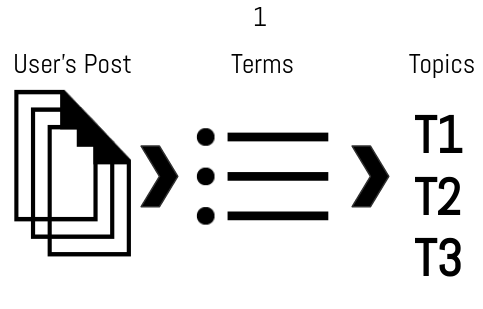
\includegraphics[scale=.5]{figs/method_1.png}
    \hspace{.5cm}
    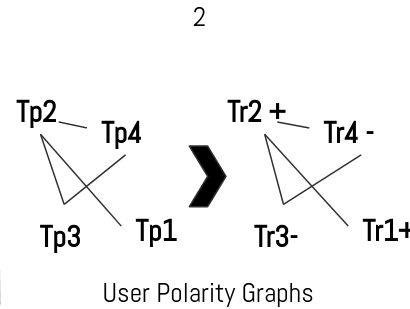
\includegraphics[scale=.5]{figs/method_2.png}\\
    \vspace{.2cm}
    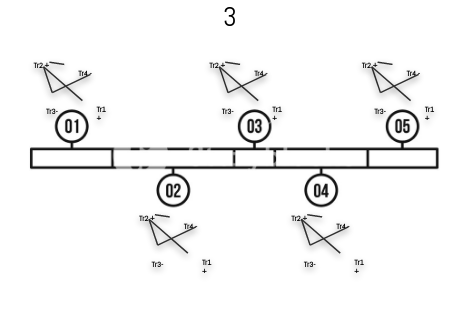
\includegraphics[scale=.6]{figs/method_3.png}
    \caption{Workflow stages for the proposed methodology}
    \label{fig:my_label}
\end{figure}

As most of the presented articles in Chapter \ref{cap:rev_literatura}, we also intend to apply text analysis over the datasets, specifically the technique that we want to employ is topic identification. Based on the work of \cite{Nolasco2016}, we aim to first identify what are the main topics of each user in a social media platform. 
After the topics identification, for each user, we could map the terms into a polarity graph. 
The polarity graph could help to identify if the most used words and terms of a user tend to be positive or negative. Related work has shown that depressive people used to manipulate more negative words. This reflects the low self-vision that this group express of themselves.
With the polarity graphs of each user, in third stage we intend to analyze how these graph have evolved over the time. In this manner, we could be capable to check if someone discourse has been turned into more positive or negative.
This could help to better explain the phenomena of depression inside social media. The time series analysis seems to be important, given that someone is considered depressed if he has manifested a set of symptoms for a certain period of time.
Also, with the graph of topics, we can apply social network metrics to understand how the users are connected, and how the people around them are affected by their discourse or behavior.

In the psychological approach, we intend to apply well defined questionnaires from psychometrics area on users selected from the computational approach. 
Psychometrics represent the theory and technique of measuring mental processes and it is applied in the fields of psychology and education. These questionnaires could be incorporated to social media users to corroborate the classification of potential users with depression.

\section{Expected Contributions}

This work still in development of methodology, with some ideas of analysis that could be made. 
The expected contributions are related to computer science and psychology.
For the computer science, we expect that employing computational metrics like social network analysis and topic classification could support people to acquire a more proper understanding of how the phenomena of depression happen in social media, and also how the social media reflects the real life. 
For the health research point of view (psychology, medicine), our approach could improve how the diagnosis of depression is performed. This could aid people with few resources to enjoy a better health by the use of technology.